\documentclass[a4paper]{article}
\usepackage[
    top=2cm,
    bottom=2cm,
    left=2cm,
    right=2cm
]{geometry}
\usepackage{fontspec}
\usepackage{xcolor}
\usepackage{graphicx} 
\usepackage{ragged2e}
\usepackage{fancyhdr}
\usepackage{tikz}
\XeTeXlinebreaklocale "km"
\XeTeXlinebreakskip = 0pt plus 1pt
\definecolor{TextBlue}{rgb}{0.1,0.2,0.7}
\baselineskip=14pt
\newcount\LineCount
\def\CountLines{\vadjust{\global\advance\LineCount by 1}}
\newfontfamily\NormalFont[
    Path=fonts/,
    Extension=.ttf
]{KhmerMPTC}
\newfontfamily\HeaderFont[
    Path=fonts/,
    Extension=.ttf
]{KhmerMPTCMoul}

\begin{document}

{\HeaderFont
\begin{center}
\fontsize{12pt}{10pt}\selectfont %random from font: 12 -> 14 , baseline spacing: it measure between its to other : 10,15,20
\textbf{ព្រះរាជាណាចក្រកម្ពុជា}\\
\textbf{ជាតិ សាសនា ព្រះមហាក្សត្រ}\\
\includegraphics[width=2.5cm]{Figures/Tacteng.png} 

\end{center}
}

\hspace*{2cm}  % random from 0,0.5,1,1.5,2
\includegraphics[width=3cm]{Figures/Mptc_logo.jpg}  % random from 2,2.5,3

{\HeaderFont
\fontsize{12pt}{10pt}\selectfont  % random from font: 10,11,12 , baseline spacing: it measure between its to other : 10,15,20
\textcolor{TextBlue}{\textbf{ក្រសួងប្រៃសណីនិងទូរគមនាគមន៍}}
}

{\NormalFont
\fontsize{11pt}{13pt}\selectfont
លេខ: ......................................... \hfill
ថ្ងៃ    ខែ      ឆ្នាំរោង ឆស័ក ព.ស ២៥៦៨
}

\raggedleft
{\NormalFont
\fontsize{12pt}{24pt}\selectfont
រាជធានីភ្នំពេញ ថ្ងៃ    ខែ    ឆ្នាំ២០២៤
}


{\HeaderFont
\begin{center}
\fontsize{12pt}{10pt}\selectfont
\textbf{សេចក្ដីជូនដំណឹងស្ដីពី}\\
\parbox{0.9\textwidth}{
\centering
\textbf{ស្តីពីវឌ្ឃនភាពនៃវិធានការរបស់វិទ្យាស្ថានបច្ចេកវិទ្យាកម្ពុជាពាក់ព័ន្ធនឹងករណីក្លែងបន្លំសញ្ញាបត្រ}%
}
\end{center}
}

{\NormalFont
\begin{justify}
\setlength{\baselineskip}{20pt}
\hspace{1cm}\input{Text/ITC_text}
\par
\end{justify}
}

\begin{flushright}
\includegraphics[width=1.5in]{Figures/Stamp.png}
\end{flushright}

\newcommand{\ornamentdivider}{%
\begin{center}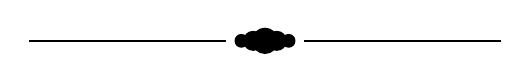
\begin{tikzpicture}
\draw[thick] (-3,0)--(-.5,0) (.5,0)--(3,0);
\foreach \x/\s in {-.3/.08,-.15/.12,0/.16,.15/.12,.3/.08}
\draw[fill=black] (\x,0) circle(\s);
\end{tikzpicture}\end{center}}

\pagestyle{fancy}
\setlength{\headheight}{0pt}
\renewcommand{\headrulewidth}{0pt}
\renewcommand{\footrulewidth}{0.4pt}
\renewcommand{\footrule}{\hbox to\headwidth{\color{TextBlue}\leaders\hrule height\footrulewidth\hfill}}

\fancyfoot[L]{
\fontsize{10pt}{10pt}\NormalFont\color{TextBlue}\selectfont
\begin{tabular}{l}
អគារលេខ ១៣ មហាវិថីព្រះមុនីវង្ស សង្កាត់ស្រះចក \\
ខណ្ឌដូនពេញ រាជធានីភ្នំពេញ 120210
\end{tabular}
}
\fancyfoot[R]{%
\fontsize{10pt}{10pt}\NormalFont\color{TextBlue}
\begin{tabular}{r}
123 023 724 810 \\
www.mptc.gov.kh
\end{tabular}
}
\end{document}
